\documentclass[final]{beamer}
\mode<presentation>
  {
    \usetheme{Bright}
  }
  \usepackage{times}
  \usepackage{amsmath,amsthm, amssymb, latexsym}
  \usepackage[english]{babel}
  \usepackage[latin1]{inputenc}
  \usepackage[size=custom,width=74,height=140,scale=1.0,debug]{beamerposter} % dimension in centimeters


% coordserver contains a family of functions that create coordinate servers, and perform GA puts and gets.  the creation functions were not modified from the ones you gave me except I made two separate ones, one for double and one for ints.  The puts and gets are slightly more easy-to-use versions of NGA_Get and NGA_Put that return either a single value of a 2D array (I made all of my arrays 2-dimensional, with the first limit being 2, just because all of them were of that form anyway...), or, if the second array index is -1, return a whole half of the array.  Later on as I became more comfortable I started calling the NGA_Gets and puts directly, when I needed the whole array, that way I wouldn’t have to call it twice


  %%%%%%%%%%%%%%%%%%%%%%%%%%%%%%%%%%%%%%%%%%%%%%%%%%%%%%%%%%%%%%%%%%%%%%%%%%%%%%%%%
  \graphicspath{}
  \title{Non-equilibrium umbrella sampling  on Blue Gene/P using one-sided communication}
  \author{Alex Dickson$^1$, Jeff R. Hammond$^2$ and Aaron R. Dinner $^1$}
  \institute{$^1$ The University of Chicago (\texttt{adickson@uchicago.edu,dinner@uchicago.edu}) \\ $^2$ Argonne National Laboratory (\texttt{jhammond@alcf.anl.gov})}
  %%%%%%%%%%%%%%%%%%%%%%%%%%%%%%%%%%%%%%%%%%%%%%%%%%%%%%%%%%%%%%%%%%%%%%%%%%%%%%%%%
  \begin{document}
    \begin{columns}[t]

      \begin{column}{.25 \linewidth}

        \begin{block}{\Large Nonequilibrium Umbrella Sampling} \Large
	  NEUS is an umbrella sampling algorithm that is applicable to nonequilibrium systems.  It divides the phase space of a system into different regions and conducts restricted simulations within each region.
          \vskip1ex
          The NEUS algorithm provides a massively-parallel method to obtain important information about rare event dynamics in complex systems.  Application of NEUS to proteins modeled with explicit-atom force-fields (instead of the simple bead model considered here) would scale to many thousands of times the number of processors required for the molecular dynamics (MD) evaluation, \textit{hence many-petaflop simulation of rare events in proteins will soon be possible}.
        \end{block}

	\begin{block}{Examples in higher dimensions}
	  \textbf{Ising Model Under Shear}
	  \begin{columns}[t]
	    \begin{column}{.65\linewidth}
	      In the sheared Ising model, NEUS used the average magnetization of the rows as order parameters (right).  The path evolved from an arbitrary initial guess to the neighborhood of the most probable reaction path (below). 
	    \end{column}
	    \begin{column}{.25\linewidth}
	      \begin{figure}
		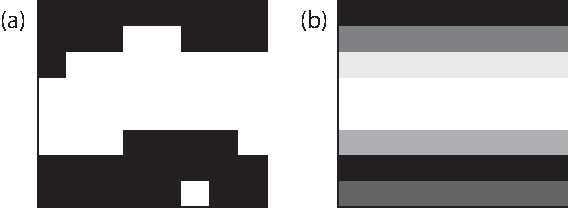
\includegraphics[width=3 in]{images/cg.pdf}
	      \end{figure}
	    \end{column}
	  \end{columns}
	  \begin{figure}
 	    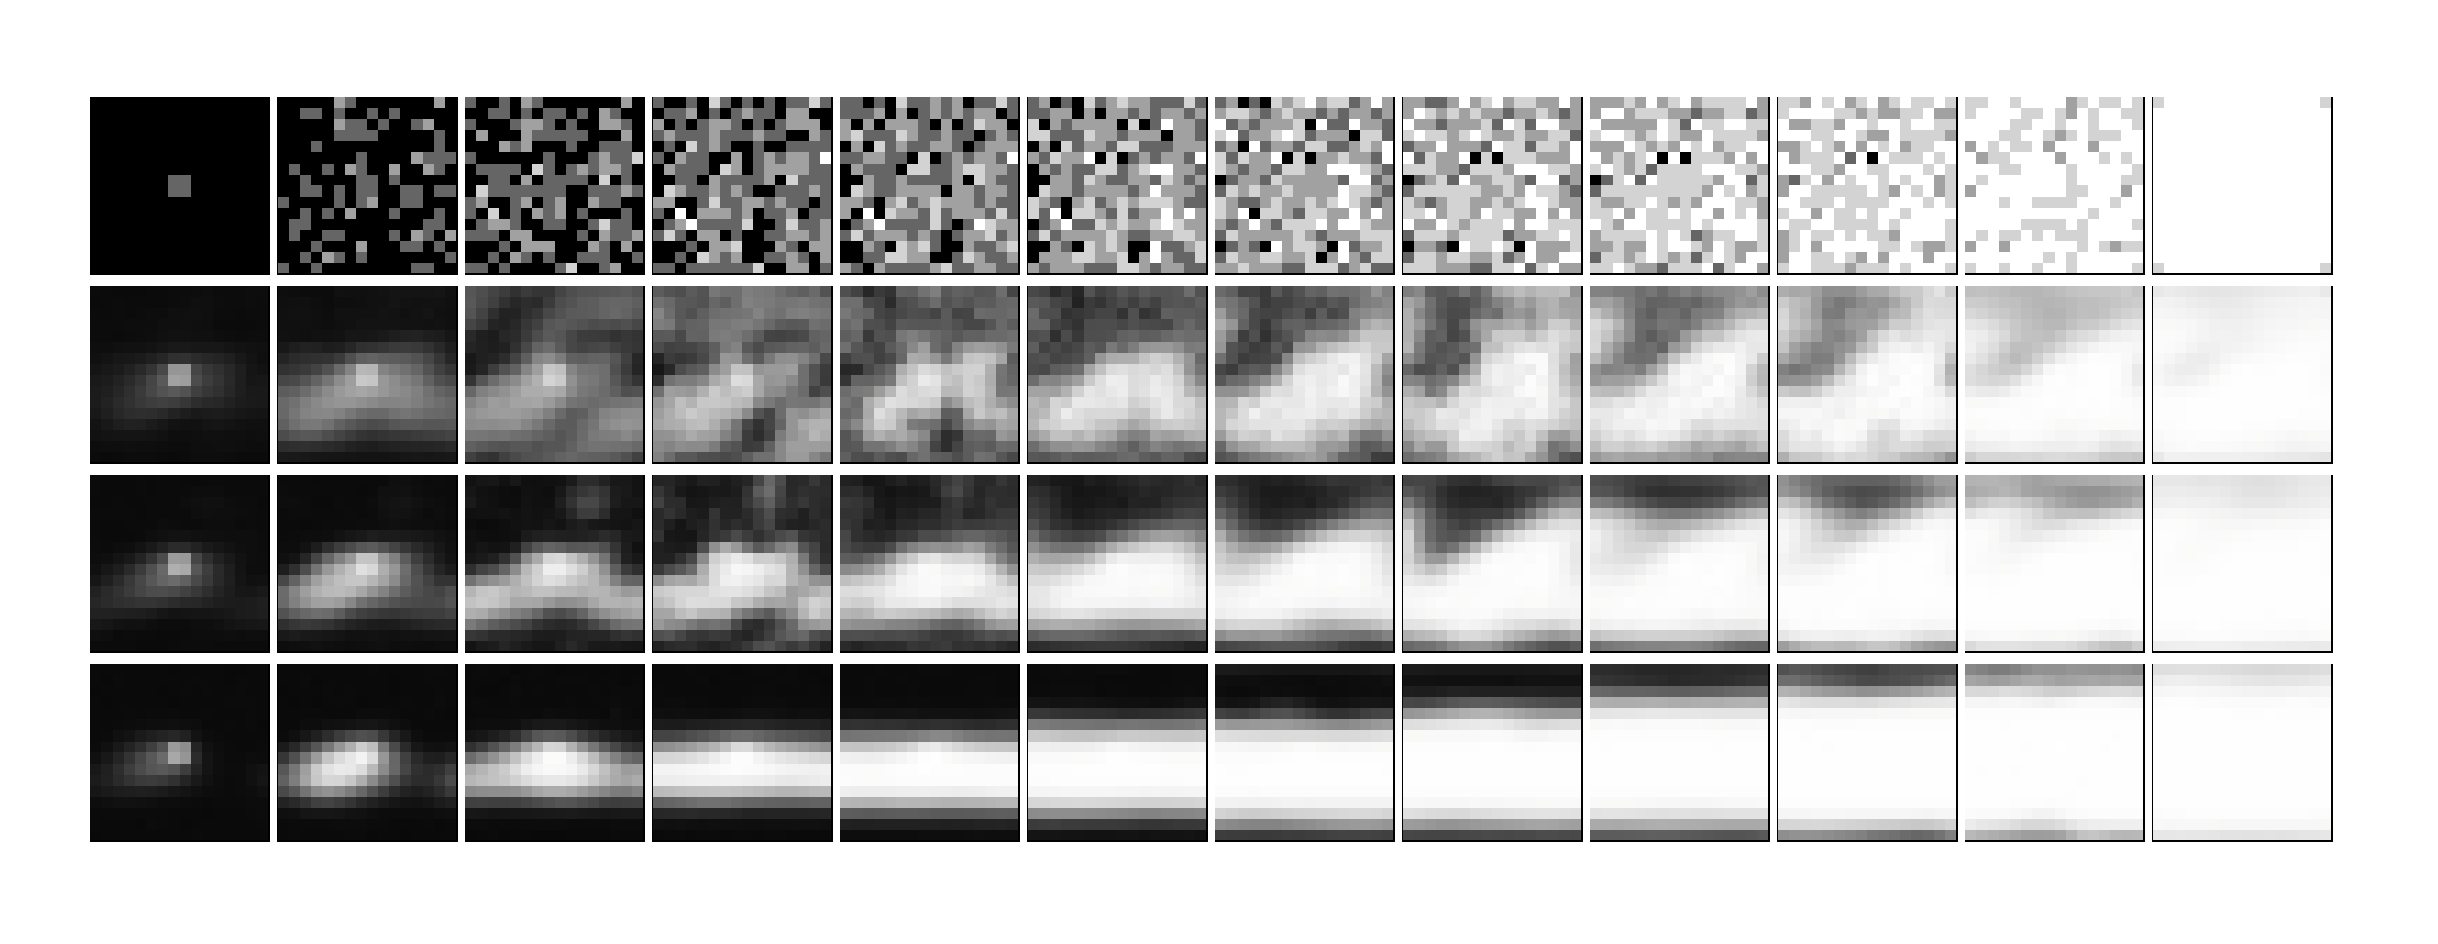
\includegraphics[width=12 in]{images/rows16.pdf}
	  \end{figure}
	  \vspace{10 mm}
	  \textbf{Circadian oscillator}

	      In a model of circadian oscillations, NEUS used the number count of each of the 22 species as order parameters.  Forward and backward path ensembles are shown below in red and blue respectively.  The algorithm was able to recover the 24h oscillatory period.
	      \begin{columns}[t]
		\begin{column}{.33\linewidth}
		  \begin{figure}
 		    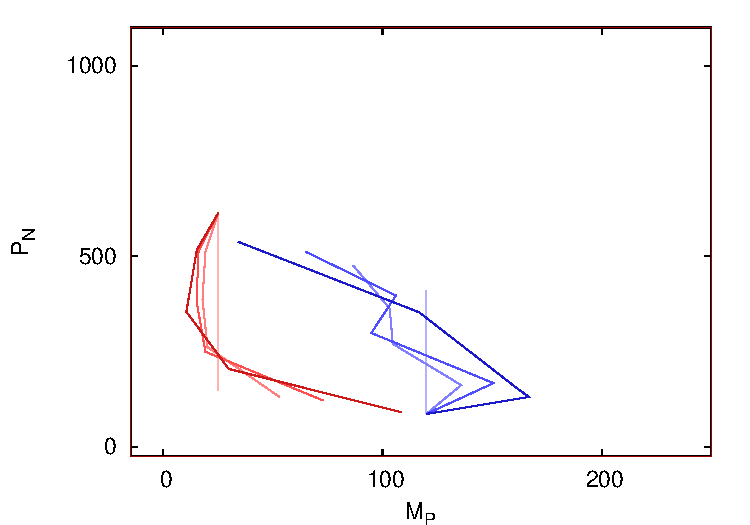
\includegraphics[width=4 in]{images/proj1umb.pdf}
		  \end{figure}
		\end{column}
		\begin{column}{.33\linewidth}
		  \begin{figure}
 		    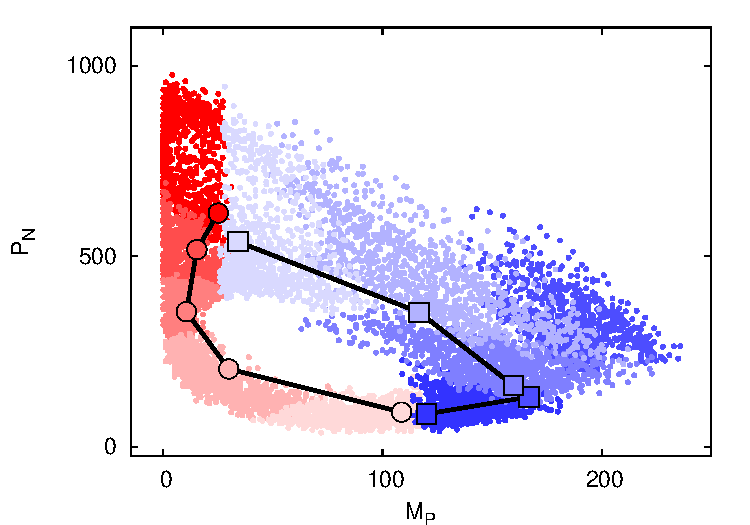
\includegraphics[width=4 in]{images/circpoints.pdf}
		  \end{figure}
		\end{column}
		\begin{column}{.33\linewidth}
		  \begin{figure}
 		    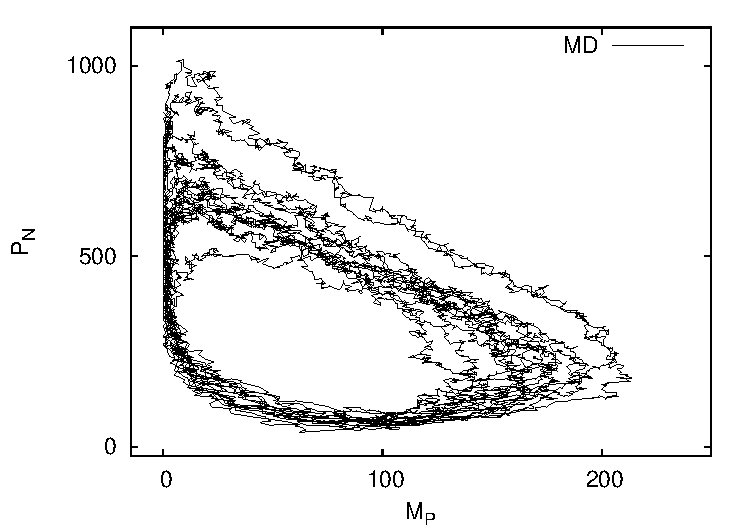
\includegraphics[width=4 in]{images/proj1md.pdf}
		  \end{figure}
		\end{column}

	  \end{columns}
        \end{block}
      \end{column}

      \begin{column}{.25 \linewidth}
%         \begin{block}{Nonequilibrium Umbrella Sampling}
% 	  NEUS is an umbrella sampling algorithm that is applicable to nonequilibrium systems.  It divides the phase space of a system into different regions and conducts restricted simulations within each region.
%           \vskip1ex
%           The NEUS algorithm provides a massively-parallel method to obtain important information about rare event dynamics in complex systems.  The scalability of NEUS \textit{improves} for larger systems since the time spent on an individual sample.  Application of NEUS to proteins modeled with explicit-atom force-fields (instead of the simple bead model considered here) would scale to many thousands of times the number of processors required for the molecular dynamics (MD) evaluation.  Given the scalability of MD codes like LAMMPS and NAMD, it is reasonable to project near-exascale simulation of rare events in proteins using explicit-atom models.
%         \end{block}
	\begin{block}{How it works}
When studying trajectories of rare events, the vast majority of computational time is spent waiting for the event of interest to happen.
NEUS is a sampling algorithm that is designed for rare events.  
It works by constructing an order parameter space using one or more degrees of freedom from the system that describe the relevant dynamics.  
This space is then divided into regions, and separate simulations are conducted within each region.  
\textbf{By enforcing sampling in every region, NEUS can simulate all stages of the event simultaneously}, and eliminate the waiting time required to see a rare event.

          \vskip1ex
	  \vspace{10 mm}
To conduct the ``regional'' simulations in nonequilibrium systems, one needs to be able to remove the bias in a physical way.
\textbf{Key insight:  run unbiased dynamics and restart walkers using a flux input distribution that is developed on-the-fly.}

	  \vspace{20 mm}

	  \begin{columns}[t]
	    \begin{column}{.4\linewidth}
	      Each region is given a weight, that is determined using boundary crossing statistics.
	      The weights are used to build the full steady-state distribution from the regional ones.
	    \end{column}
	    \begin{column}{.25\linewidth}
	      \begin{figure}
		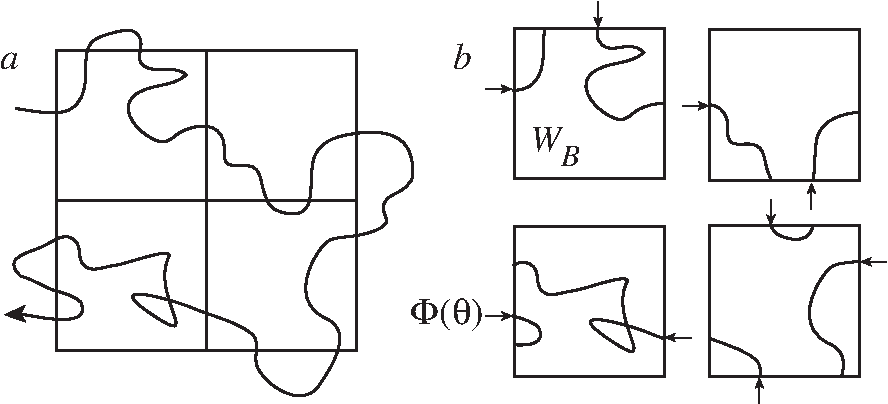
\includegraphics[width=3 in]{images/motivation2.pdf}
	      \end{figure}
	    \end{column}
	    \begin{column}{.25\linewidth}
	      \begin{figure}
		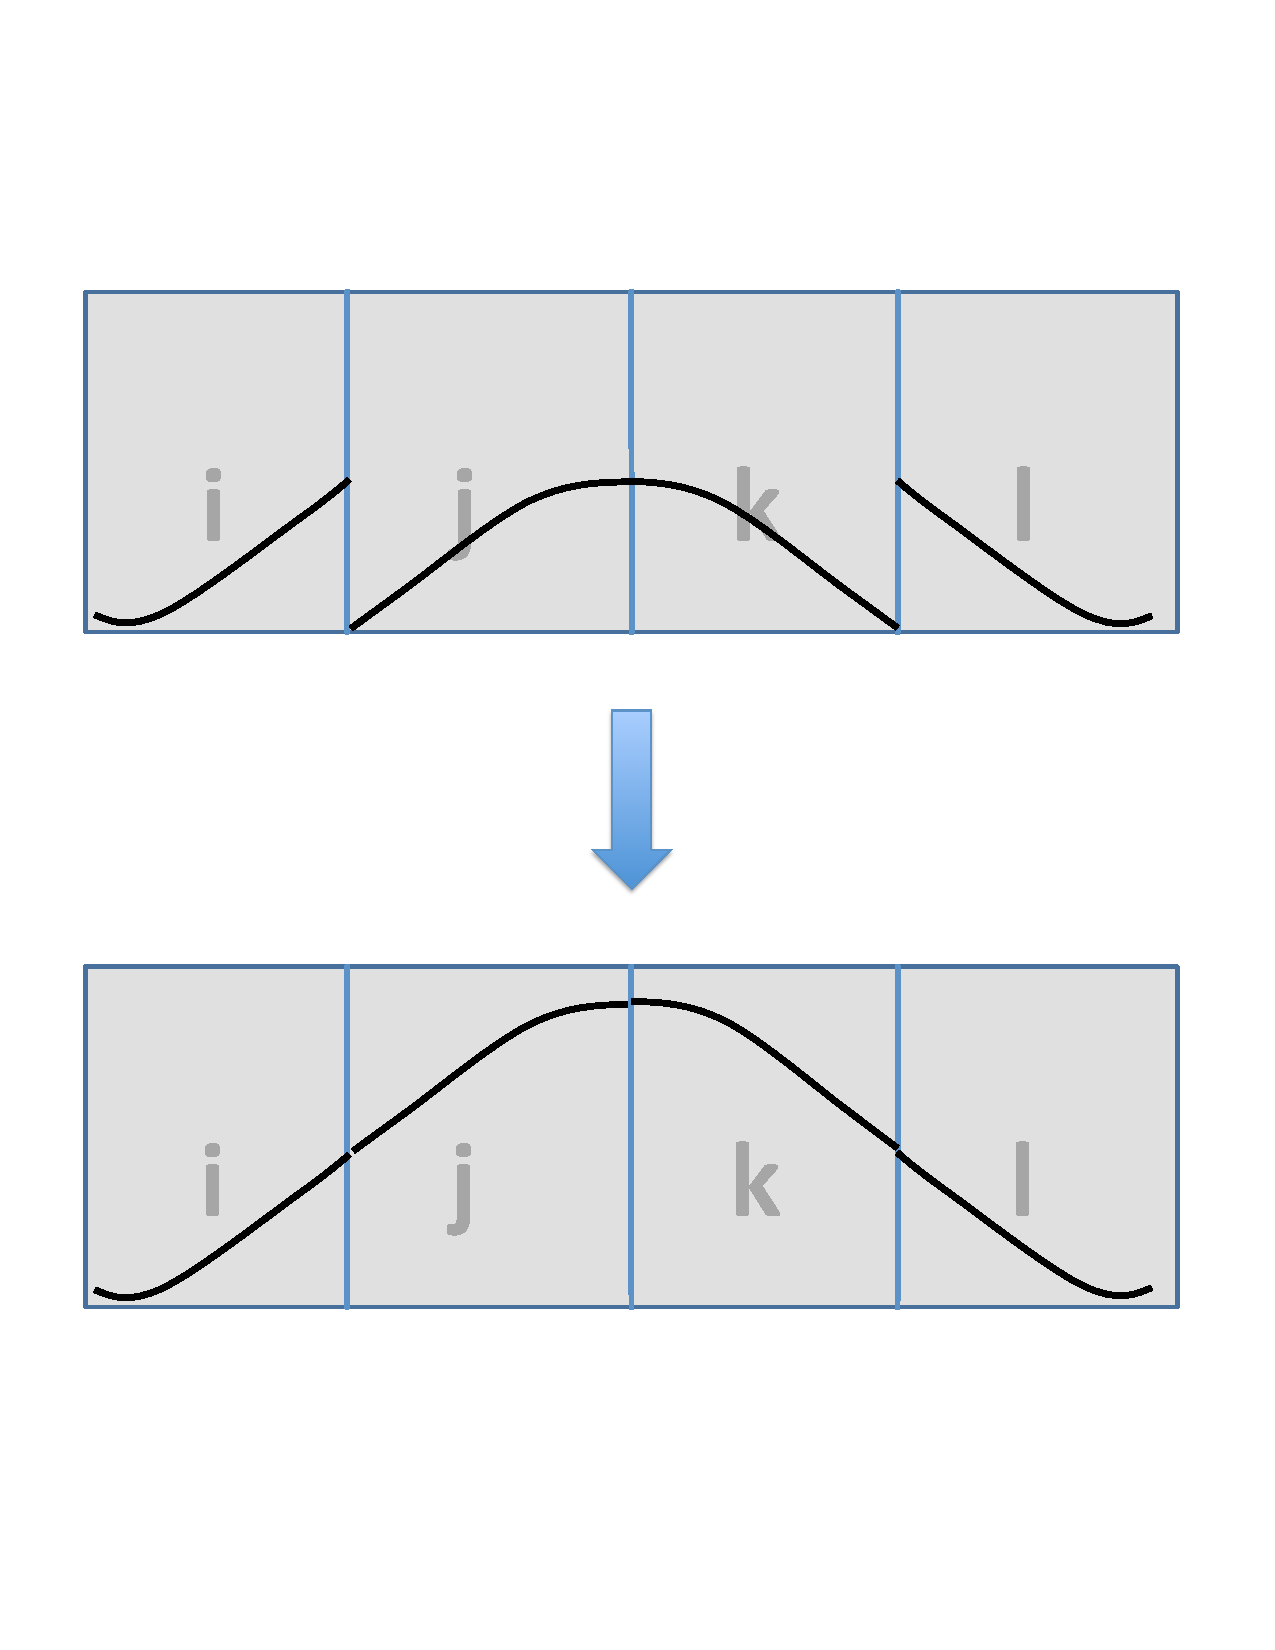
\includegraphics[width=2 in]{images/patch.pdf}
	      \end{figure}
	    \end{column}
	  \end{columns}

        \end{block}
	\begin{block}{Advanced Techniques}
	  \textbf{Strings:}

	  \begin{columns}[t]
	    \begin{column}{.65\linewidth}

	  Irregular regions can be formed by Voronoi polyhedra defined using a set of phase space points (``images'') that together form a string that winds its way from reactants to products.
	  The string is updated during sampling by periodically moving the images towards the average of the walker position in the last time interval.

	    \end{column}
	    \begin{column}{.25\linewidth}
	      \begin{figure}
		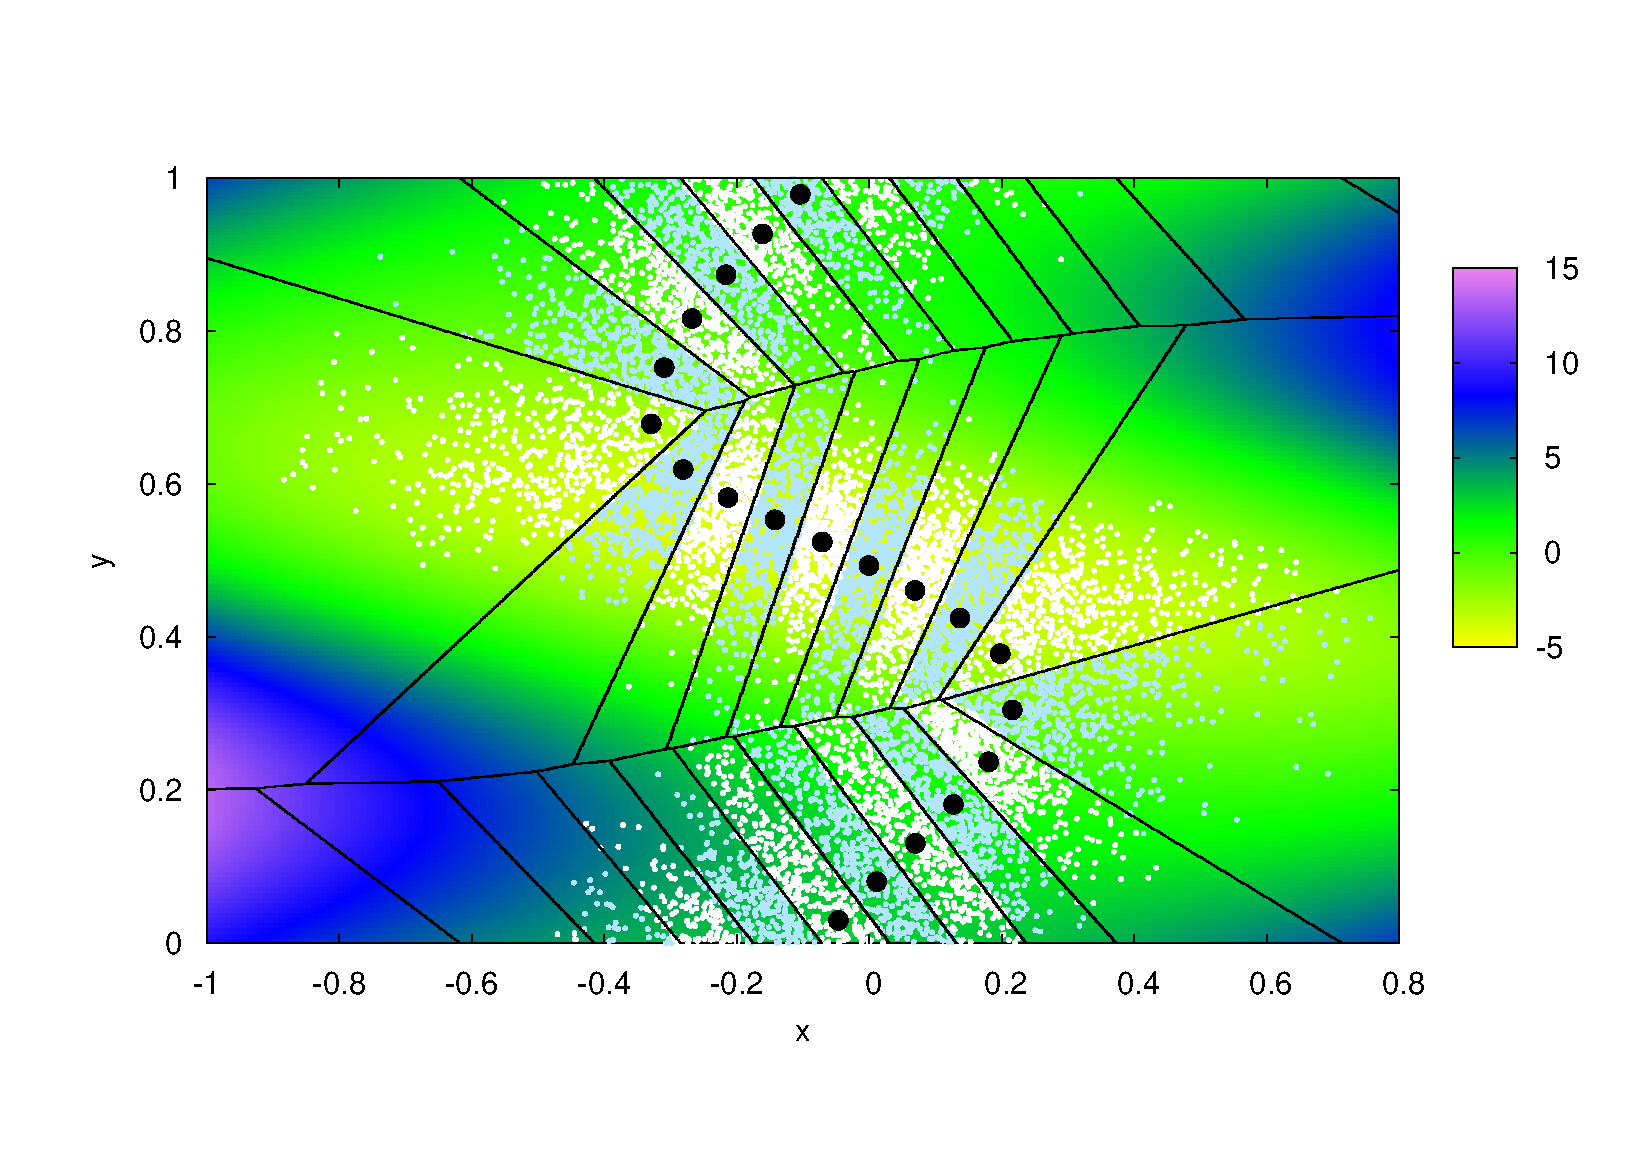
\includegraphics[width=3 in]{images/whiteandblue.pdf}
	      \end{figure}
	    \end{column}
	  \end{columns}
	  \vspace{30 mm}
	  \textbf{Separating the transition path ensemble:}

	  \begin{columns}[t]
	    \begin{column}{.65\linewidth}

	      We can also separate trajectories based on their basin of origin by defining two ensembles:  ${\cal S}_A$ for trajectories originating in basin $A$, and ${\cal S}_B$ for trajectories originating in basin $B$.
	  This allows for a better description of transition paths that are separate due to nonequilibrium path splitting, and as a bonus, it allows for the \textbf{easy calculation of transition rates!}

	  \begin{equation*}
	    \label{eq:rate}
	    k_{AB} = \frac{\overline{\Phi}_{B \mid {\cal S}_A}}{\overline{h}_A}
	  \end{equation*}

	  where $\overline{\Phi}_{B \mid {\cal S}_A}$ is the flux into basin $B$ from the ${\cal S}_A$ ensemble, and $\overline{h}_A$ is the total weight of all regions in ${\cal S}_A$.
	    \end{column}
	    \begin{column}{.25\linewidth}
	      \begin{figure}
 		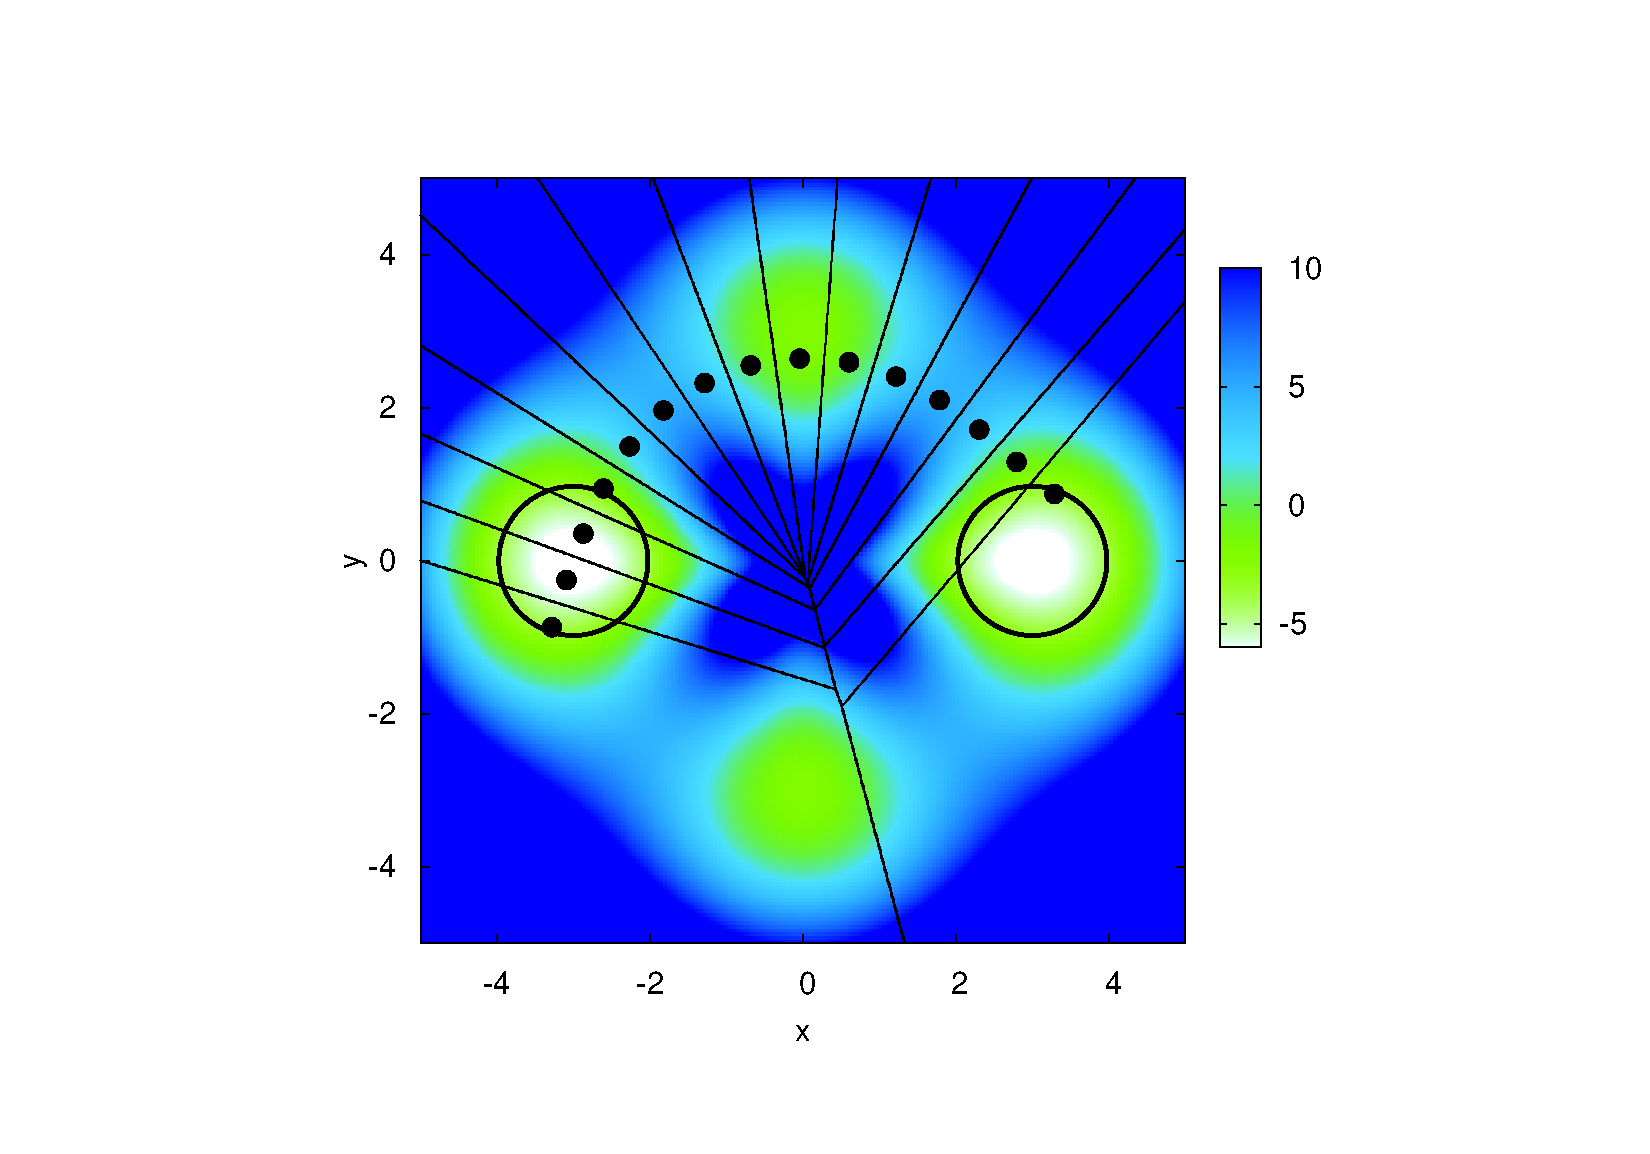
\includegraphics[width=3 in]{images/contvorf.pdf}
	      \end{figure}
	      \begin{figure}
 		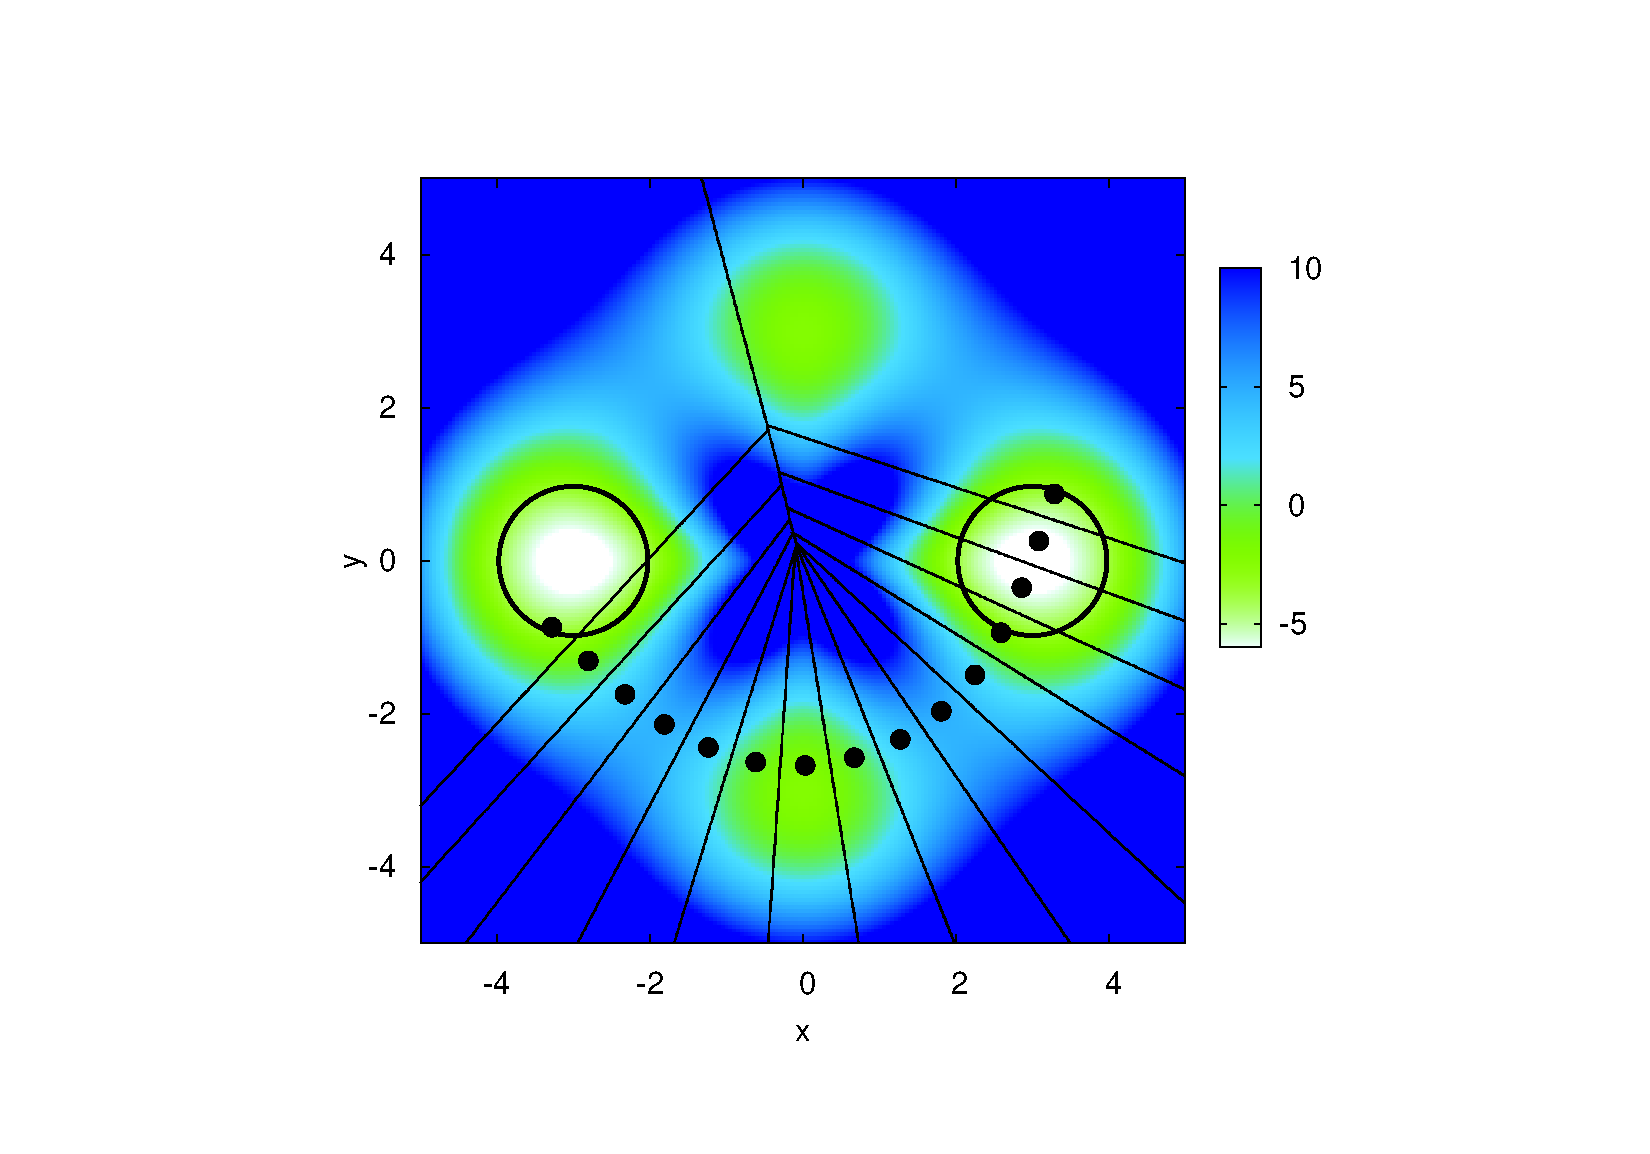
\includegraphics[width=3 in]{images/contvorr.pdf}
	      \end{figure}
	    \end{column}
	  \end{columns}
	  
        \end{block}
      \end{column}

      \begin{column}{.25 \linewidth}
        \begin{block}{Parallelization using Global Arrays}
	  \begin{columns}[t]
	    \begin{column}{.40\linewidth}
	      NEUS is best implemented using a global state variable updated by atomic (complex) operations asynchronously.  Global Arrays (GA) Put/Get operations in conjunction with Lock/Unlock provide a means to implement the necessary tools in a straightforward way.  The implementation of NEUS on top of GA is called CoordServer.
	    \end{column}
	    \begin{column}{.55\linewidth}
                \begin{figure}[hctp]
                    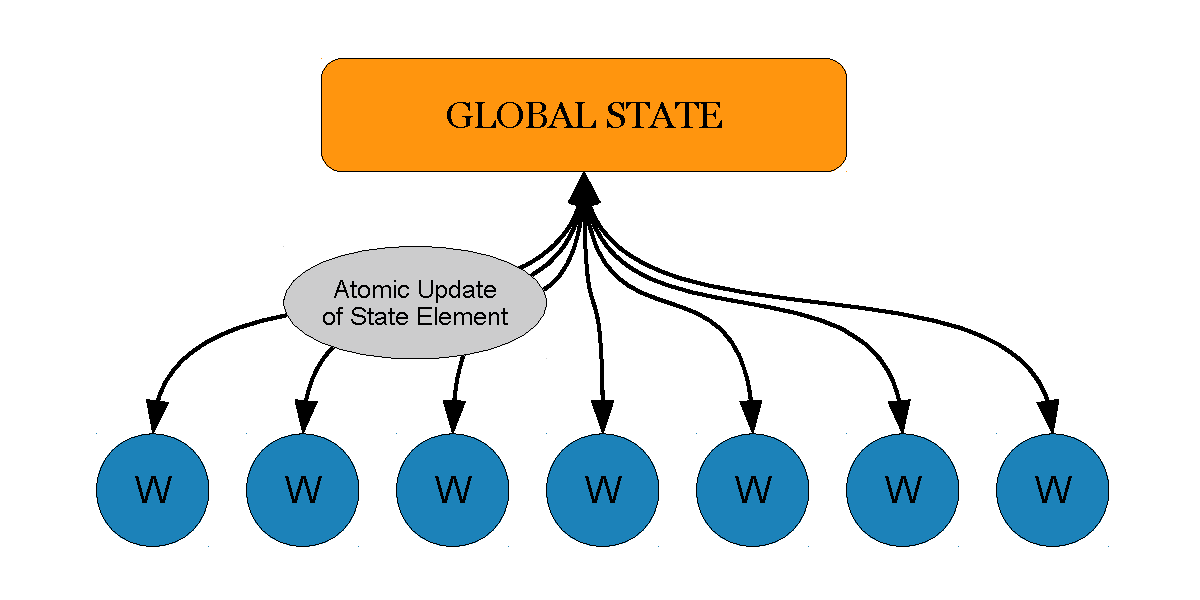
\includegraphics[width=1.0\linewidth]{images/soft_arch.pdf}
                \end{figure}
	    \end{column}
	  \end{columns}
          \vskip2ex
	  \begin{columns}[t]
	    \begin{column}{.40\linewidth}
	      Because Global Arrays provides a \textit{distributed} global state, unlike if CoordServer was implemented using a master-worker approach, atomic updates can occur simultaneously except when locked and need not wait on the master process all tasks sequentially.
	    \end{column}
	    \begin{column}{.55\linewidth}
                \begin{figure}[hctp]
%                    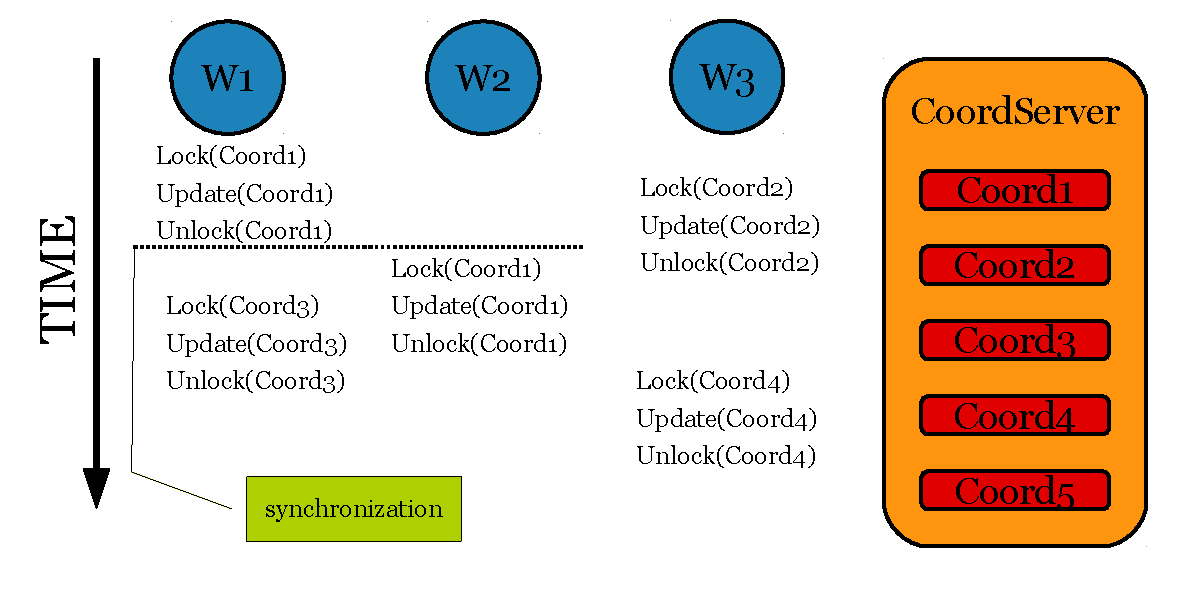
\includegraphics[width=1.0\linewidth]{images/coord_server.pdf}
                \end{figure}
	    \end{column}
	  \end{columns}
        \end{block}
        \begin{block}{Scaling on Blue Gene/P}

	  \begin{columns}[t]
	    \begin{column}{.32\linewidth}
	      The distributed nature of the NEUS global state allows for efficient strong-scaling due to the majority of asynchronous updates being nonconflicting.  Recent optimizations of Global Arrays for Blue Gene/P [Hammond et al. submitted to PGAS 2010] reduce the computation time in this loosely-coupled code signficantly.
	    \end{column}
	    \begin{column}{.65\linewidth}
                In preliminary measurements, we are able to achieve strong scaling to 8192 processors (2048 nodes on Blue Gene/P) with 96\% efficiency.
                \begin{figure}[hctp]
                    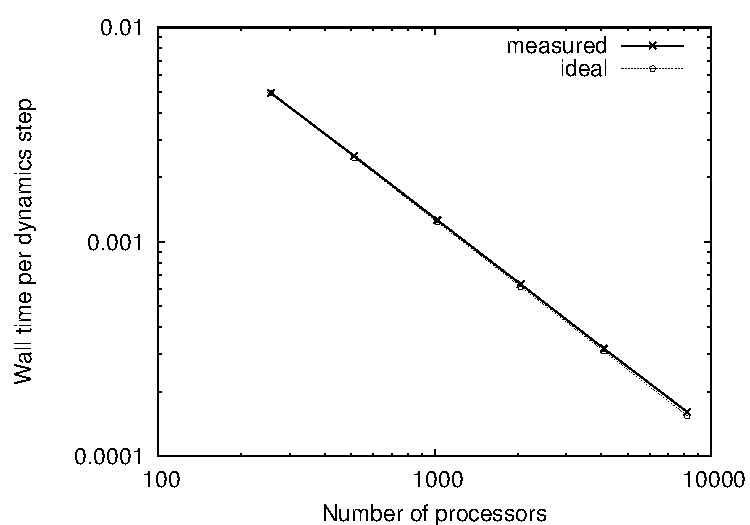
\includegraphics[width=1.0\linewidth]{images/scale.pdf}
                \end{figure}
	    \end{column}
	  \end{columns}
          {\color{red} TO BE ADDED LATER:} \\
          {\color{red} 1.} OpenMP parallelism has been implemented already.  New performance results will be added to the final version of the poster.  In addition, we will run scaling tests on at least 16K nodes. \\
          {\color{red} 2.} Detailed breakdown of computation and communication timings in the code at various scales.  Extensive TAU performance analysis has already been performed on the code, we just need to rerun with the latest version.
        \end{block}
      \end{column}

      \begin{column}{.25 \linewidth}
        \begin{block}{Preliminary Results for a large RNA molecule under flow}
	  Each of the 262 nucleotides is represented by a single bead.  Adjacent beads in the chain are connected with a FENE potential, and secondary and tertiary interactions are modelled with a Lennard-Jones potential.  There are also repulsive terms to keep the chain locall straight, and to mimic steric repulsion.  The flow is simulated with the stochastic rotation dynamics method.  Each step of the algorithm is comprised of a free streaming step and a ``collision'' step in which the velocity of each particle in the cell is rotated around the cell's average velocity vector by a random rotation matrix.
          \vskip1ex
	  \vspace{10 mm}
	  The flow is simulated with the stochastic rotation dynamics method
	  %\cite{Malevanets1999,Ihle2001,Lamura2001,Allahyarov2002}.
          In that method, the solvent is represented by a large number of infinitesimal particles that are grouped into cells of a lattice.  Each step of the algorithm is comprised of a free streaming step and a ``collision'' step in which the velocity of each particle in the cell is rotated around the cell's average velocity vector by a random rotation matrix.

	  The RNA beads are included in the collisions, through which the solvent will influence the polymer.
	  \vspace{10 mm}

	  \begin{columns}[t]
	    \begin{column}{.45\linewidth}
	      \textbf{Evidence for long-lived stable-states}: The competition between the flow and the native contacts results in a rich dynamics that includes competing metastable states.  We are interested in the intermediate case, where contracted and extended states coexist, and transitions between them occur on long, macroscopic timescales.
              \vskip1ex
	      Straight-forward trajectories show evidence of these long-lived meta-stable states.  
	      These trajectories were run on a single processor for 24 hours each (2 $\mu$s, with a 0.4 ps time step), and over that time did not exit their respective basins, revealing the presence of competing metastable states.
	    \end{column}
	    \begin{column}{.50\linewidth}
	      \begin{figure}[hctp]
                \vskip -2ex
                \caption{Extension vs. time for two trajectories with different initial conditions.}
		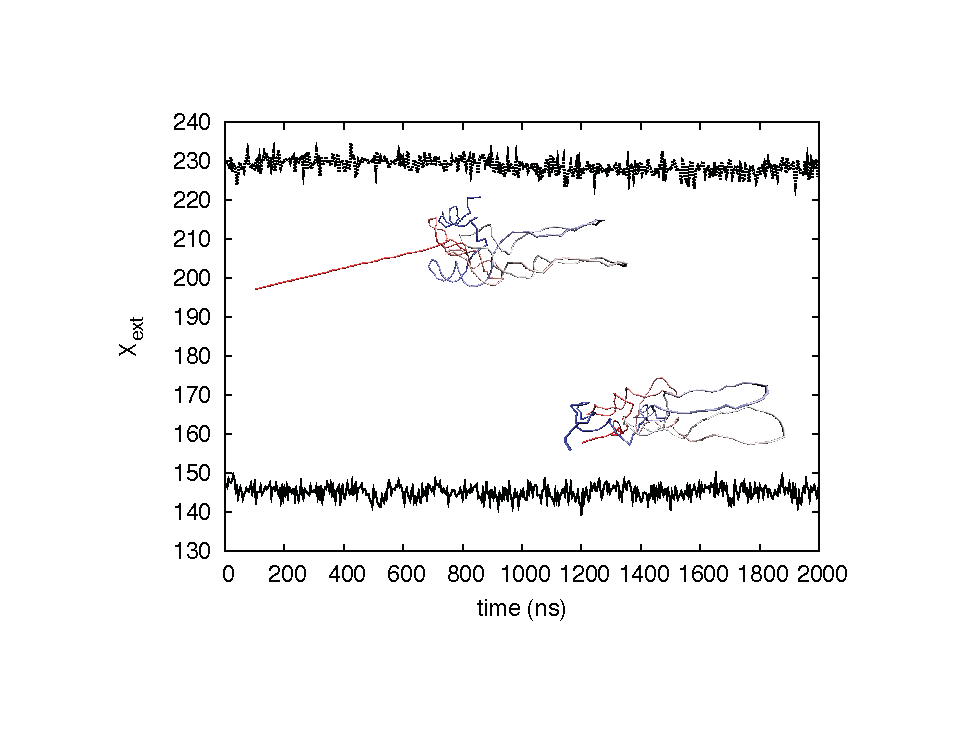
\includegraphics[width=1.0\linewidth]{images/ext_fig.pdf}
	      \end{figure}
	    \end{column}
	  \end{columns}
          \vskip2ex
          {\color{red} TO BE ADDED LATER:} The scientific analysis will be completed in conjunction with a scientific journal submission.  The current write-up is quite crude.
        \end{block}
      \end{column}


    \end{columns}
  \end{document}